% Audited anonymous initial-submission source for ICLR 2027.
\documentclass{article}
\usepackage{iclr2027_conference,times}
\usepackage[utf8]{inputenc}
\usepackage[T1]{fontenc}
\usepackage[hidelinks]{hyperref}
\usepackage{url}
\usepackage{booktabs}
\usepackage{amsfonts}
\usepackage{amsmath}
\usepackage{xcolor}
\usepackage{graphicx}
\usepackage{enumitem}
\usepackage{multirow}
\usepackage{microtype}

\newcommand{\cer}{\textsc{CER-Bench}}
\newcommand{\agent}{\textsc{Agent}}

\title{CER-Bench: Diagnosing Condition-Sensitive Evidence Retrieval in Biomedical Literature}
\author{Anonymous Authors}

% Anonymous initial submission: keep \iclrfinalcopy commented out.
% \iclrfinalcopy

\begin{document}
\maketitle

\begin{abstract}
We introduce \cer, a diagnostic benchmark for condition-sensitive evidence retrieval in biomedical literature. Its 304 corpus-grounded tasks span eight families: constraint satisfaction, comparison, contradiction, abstention, multi-hop retrieval, temporal synthesis, aggregation, and negative-result retrieval. The search corpus contains 4,936 papers and 17,902 scientific-structure chunks across ten biomedical subdomains. We evaluate eleven primary configurations---BM25, four dense retrievers, SPLADE, hybrid fusion, two rerankers, and one- and three-round search agents---plus an RM3 diagnostic. The central result is not a universal winner but pronounced \emph{evaluation sensitivity}. On 108 non-abstention test tasks with 2.4 seed relevance judgments per query, BM25 leads MRR (0.566), SPLADE is the strongest single-pass system at R@20 (0.517), and the three-round agent reaches 0.543 R@20. After pooling and LLM-adjudicating systems' top-20 results, BGE leads R@20 (0.416) while the agent ranks fifth (0.352). On 70 test tasks with higher-density cluster-proxy qrels, BM25 also exceeds the agent (0.449 vs.\ 0.376 R@20). Iteration nevertheless raises agent R@20 from 0.299 to 0.543 under seed judgments. No evaluated retriever abstains on any of 17 unsupported queries. These findings show that task structure and relevance-judgment construction can change conclusions as much as retriever choice, motivating explicit qrel audits and human validation for scientific-search benchmarks.
\end{abstract}

\section{Introduction}
\label{sec:intro}

Scientific search often requires more than topical similarity. A researcher may need papers satisfying several experimental conditions simultaneously, evidence on both sides of a comparison, a chain distributed across papers, or every reported value for a measurement. The system should also recognize when its corpus cannot support a question. Standard retrieval metrics can hide these distinctions by reducing each query to an undifferentiated set of relevant documents.

Existing scientific-search benchmarks expose parts of this problem. DORIS-MAE evaluates multi-aspect scientific queries and reports substantial degradation across seventeen retrievers~\cite{dorismae2023}; LitSearch collects realistic literature-search questions~\cite{litsearch2024}; and EpiBench studies multi-turn multimodal research workflows~\cite{epibench2026}. BioASQ, TREC Precision Medicine, SciFact, and BEIR provide influential biomedical or cross-domain test collections~\cite{bioasq2015,trecpm2017,scifact2020,beir2021}. These resources are valuable, but none jointly separates the eight evidence-collection capabilities in Figure~\ref{fig:taxonomy} or treats unsupported questions as a first-class family.

The relevance judgments (qrels) used to evaluate such systems are equally important. Incomplete judgments can change system rankings~\cite{buckley2004incomplete}, and relevance itself varies across assessors~\cite{voorhees2000judgments}. This issue is acute when queries are synthesized from a small seed set: the generating papers are known to be relevant, but other relevant papers remain unjudged. \cer therefore reports three deliberately different qrel constructions rather than presenting any one as complete ground truth.

\begin{figure*}[t]
  \centering
  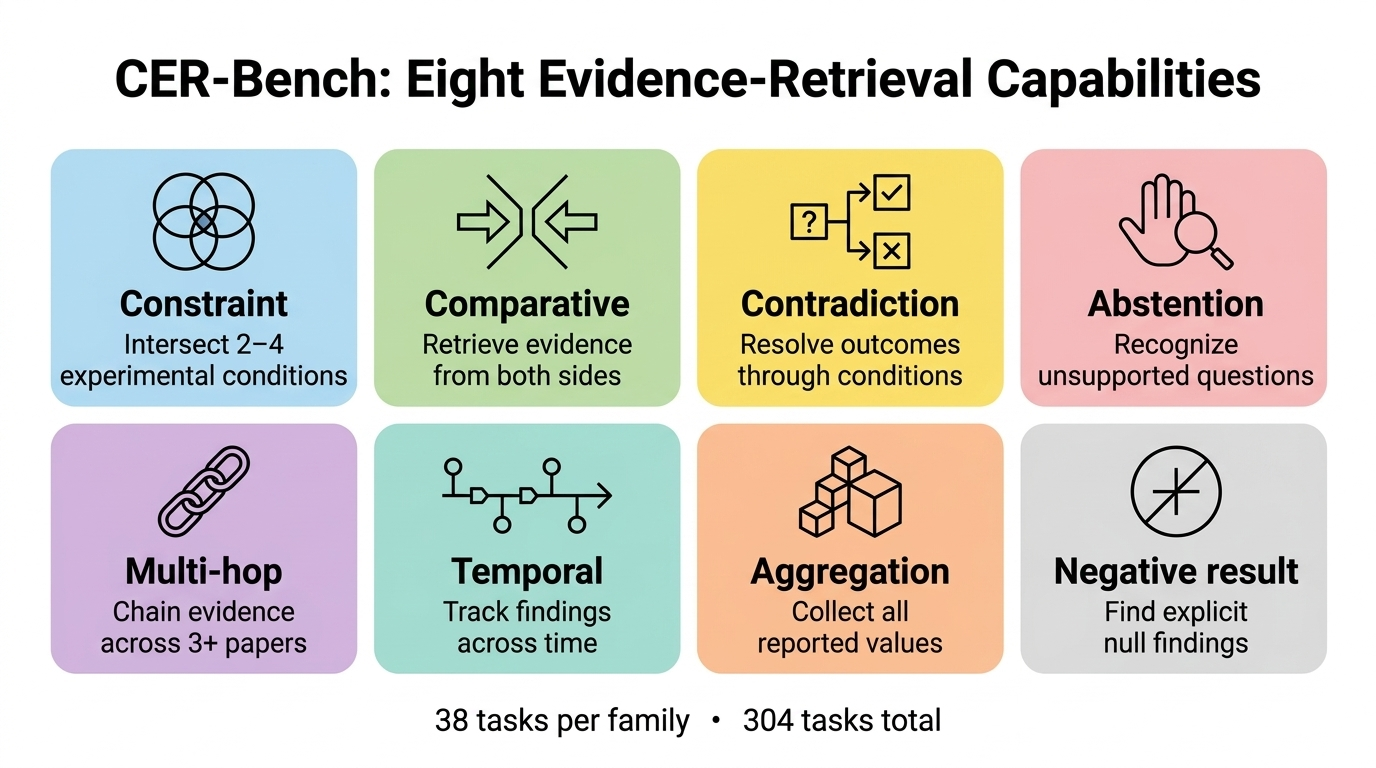
\includegraphics[width=0.94\textwidth]{figures/task_taxonomy_redesign.png}
  \caption{The eight \cer task families. Each family isolates a different evidence-collection requirement; all contain 38 tasks. Color and icon shape provide redundant encoding. Exact definitions and examples appear in Appendix~\ref{app:taskdetails}.}
  \label{fig:taxonomy}
\end{figure*}

Our contributions are fourfold:
\begin{itemize}[leftmargin=*,itemsep=2pt,topsep=2pt]
  \item We introduce 304 corpus-grounded biomedical retrieval tasks balanced across eight capability families, paired with a 4,936-paper corpus and explicit unsupported-query cases.
  \item We evaluate eleven primary retrieval configurations plus an RM3 diagnostic, including lexical, dense, learned-sparse, fusion, reranking, and iterative-search approaches under a common document-level protocol.
  \item We audit conclusion stability across seed qrels, pooled LLM-adjudicated qrels, and higher-density cluster-proxy qrels. The resulting ranking reversals are the paper's main empirical finding.
  \item We provide an artifact-driven integrity audit that recomputes headline metrics, paired-bootstrap intervals, split overlap, adjudication counts, and figures from saved outputs; we also state where human evidence is absent.
\end{itemize}

\section{Related Work}
\label{sec:related}

\paragraph{Scientific retrieval and synthesis.}
SPECTER2 learns task-format-specific scientific document representations~\cite{specter2}. OpenScholar combines retrieval over 45 million papers with an 8B language model for scientific question answering~\cite{openscholar2026}, while PaperQA2 targets end-to-end literature synthesis~\cite{skarlinski2024paperqa2}. These systems motivate strong scientific-search infrastructure, but answer-generation quality does not isolate retrieval failures. \cer evaluates retrieved evidence sets directly.

\paragraph{Iterative retrieval.}
Context-1 trains a self-editing search agent with decomposition, retrieval, pruning, and refinement~\cite{context2026}; Chain of Retrieval studies multi-aspect expansion and aggregation for full-paper retrieval~\cite{cor2025}. Our controller is intentionally narrower: it repeatedly queries a fixed BM25 index and accumulates unique documents, without learned pruning, graph traversal, or score fusion. This makes iteration itself the ablated variable.

\paragraph{Retrieval evaluation.}
Pooling is a standard response to incomplete qrels, but systems outside a pool can still discover unjudged relevant documents~\cite{buckley2004incomplete}. LLM judges offer scalable annotation, yet documented position, verbosity, and self-enhancement biases caution against treating them as human ground truth~\cite{zheng2023judge}. We consequently use pooled LLM judgments only as a sensitivity analysis and identify the absence of independent human adjudication as the benchmark's primary limitation.

\section{CER-Bench}
\label{sec:benchmark}

\subsection{Corpus}

We build the corpus from PubMed metadata and MeSH terms~\cite{pubmed_nlm}, PubMed Central Open Access full text~\cite{pmc_nlm}, and OpenAlex citation and topic metadata~\cite{openalex2022}. Ten seed searches cover CRISPR, checkpoint immunotherapy, drug repurposing, CAR-T therapy, organoids, single-cell methods, the microbiome, mRNA therapeutics, protein-structure prediction, and epigenetics. After English-language and publication-type filtering, the corpus contains 4,936 papers from 2015--2026. Of these, 652 have parsed PMC full text and 4,284 are abstract-only. Scientific-structure chunking produces 17,902 chunks (median 304 tokens; 6.59M estimated tokens). Appendix~\ref{app:corpus} gives exact composition and processing details.

\subsection{Task Families}

\begin{table*}[t]
\centering
\caption{Task-family definitions. Each family contains 38 tasks (304 total).}
\label{tab:families}
\small
\begin{tabular}{@{}lp{0.32\textwidth}lp{0.32\textwidth}@{}}
\toprule
\textbf{Family} & \textbf{Retrieval requirement} & \textbf{Family} & \textbf{Retrieval requirement} \\
\midrule
Constraint & Satisfy all stated organism, assay, intervention, outcome, or time constraints. & Multi-hop & Recover a chain of evidence distributed across at least three papers. \\
Comparative & Retrieve evidence representing both sides of a specified comparison. & Temporal & Cover evidence from multiple periods to trace change over time. \\
Contradiction & Retrieve opposing findings and the conditions that reconcile them. & Aggregation & Collect reported quantities or findings across multiple studies. \\
Abstention & Return no evidence when no corpus document satisfies all constraints. & Negative & Surface explicit null, non-significant, or failed-replication findings. \\
\bottomrule
\end{tabular}
\end{table*}

Each task stores a natural-language question, structured constraints, task family, supporting document identifiers, and hard-negative identifiers where applicable. The benchmark is retrieval-only: reference answers guide construction but are not scored. For comparative, contradiction, temporal, multi-hop, and aggregation queries, plain Recall@$k$ is an incomplete proxy for satisfying the requested structure; we therefore report family-specific breakdowns and avoid claiming that aggregate recall fully measures task success.

\subsection{Construction and Three Qrel Regimes}
\label{sec:qrels}

\paragraph{Seed qrels (v1).}
For each non-abstention task, we sample 2--3 related corpus papers and prompt Claude Sonnet 4 to generate a family-specific query using their titles, abstracts, and metadata. The sampled documents become \emph{seed qrels}; they are verified members of the construction context, not an exhaustive relevance set. Abstention queries combine plausible constraints not jointly satisfied by the sampled near-miss papers and receive an empty qrel set. We generate 38 tasks per family and stratify them into 119/60/125 train/dev/test tasks; 108 test tasks have non-empty qrels. The controller prompt was refined on development tasks before the test split was evaluated.

\paragraph{Pooled qrels.}
For each of the 108 non-abstention test queries, we pool unique documents from the top 20 of nine primary non-agentic systems and the three-round agent. Seed documents are retained as relevant. Claude Sonnet 4 independently receives the query, structured constraints, and candidate text, but not method identity or rank, and returns a binary verdict plus supporting span. Prefix-normalizing the saved verdict strings yields 1,106 relevant and 2,134 non-relevant judgments (3,240 total); qrels expand from 2.4 to 12.7 documents/query on average (range 2--31). Because the task generator and judge use the same model family and no human adjudication is available, pooled qrels are a robustness view rather than a gold standard.

\paragraph{Cluster-proxy qrels (v2).}
As a second stress test, BM25 retrieves candidates around a seed paper, Sonnet filters papers for topic-level relation to that seed, and Sonnet then generates one query from the resulting 6--16-paper cluster. Every cluster member is assigned as a proxy relevant document. This produces 200 balanced tasks; reported retrieval results use the 70 non-abstention test tasks for which agent outputs are saved. Cluster membership is \emph{not} document-level verification against the final query and is not exhaustive. We therefore call these \emph{cluster-proxy qrels}, correcting the stronger ``complete gold'' interpretation suggested by the generation script.

\paragraph{Split audit.}
The task-level split is not document-disjoint: 26 of 125 test tasks share at least one supporting document with train or development, and two test questions exactly duplicate training questions. Main systems are not trained on \cer, but development-time prompt selection can still exploit shared structure. We report an 82-task document-disjoint non-abstention sensitivity slice in Appendix~\ref{app:split}.

\section{Retrieval Systems and Evaluation}
\label{sec:methods}

We compare eleven primary configurations. \textbf{Lexical:} BM25 ($k_1{=}1.2$, $b{=}0.75$)~\cite{robertson2009}. \textbf{Dense:} SPECTER2, BGE-base-en-v1.5, E5-large-v2, and MedCPT~\cite{specter2,bge2024,e52022,medcpt2023}, using exact inner-product search in FAISS~\cite{johnson2019faiss}. \textbf{Learned sparse:} SPLADE with the public \texttt{naver/splade-cocondenser-ensembledistil} checkpoint~\cite{splade2022}. \textbf{Fusion and reranking:} reciprocal-rank fusion (RRF, $k{=}60$) of BM25 and SPECTER2~\cite{rrf2009}; an MS-MARCO MiniLM cross-encoder over the top-50 hybrid chunks~\cite{nogueira2019bert}; and BGE-reranker-v2-m3 over BM25's top 50. \textbf{Iterative:} the same Sonnet controller with one or three search rounds. BM25+RM3 is an additional pseudo-relevance-feedback diagnostic~\cite{abduljaleel2004rm3}, yielding twelve rows in the main table.

At each controller round, Sonnet receives the original query, accumulated evidence, and eight previously unseen BM25 chunks with titles and snippets. It either issues a refined subquery or stops with selected document identifiers. At the three-round limit, all accumulated unique documents are returned in retrieval order, capped at 20; no score fusion is applied. The exact prompt and architecture schematic appear in Appendix~\ref{app:controller}.

\begin{figure}[t]
  \centering
  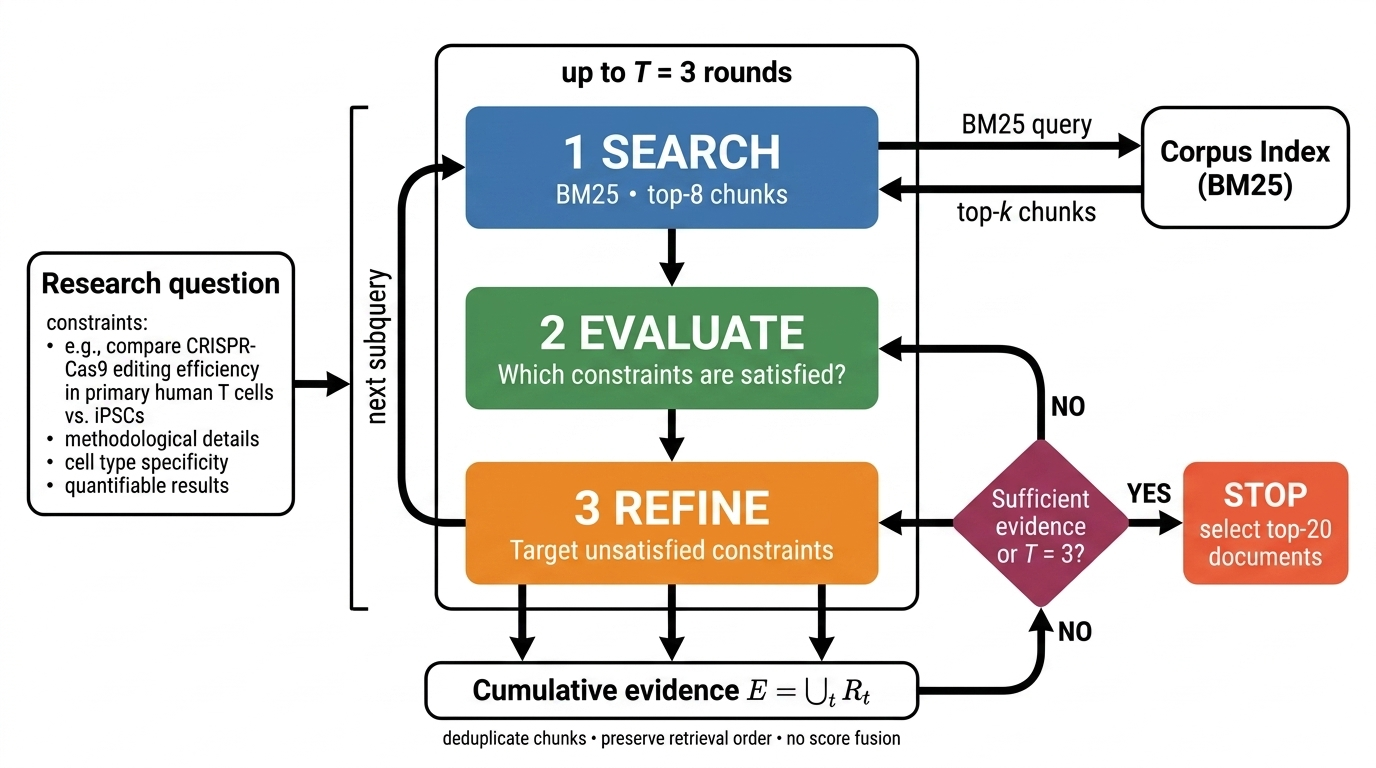
\includegraphics[width=\linewidth]{figures/agent_architecture_redesign.png}
  \caption{Iterative controller. The model sees eight new BM25 chunks per round, evaluates unmet constraints, and either refines or stops. Documents are deduplicated across at most three rounds; no cross-round score fusion is used.}
  \label{fig:controller}
\end{figure}

All systems are scored at document level after chunk deduplication. We report Recall@$k$ for $k\in\{5,10,20\}$, nDCG@10, and MRR. Empty-qrel abstention tasks are excluded from retrieval averages and evaluated separately. For key v1 comparisons we use 10,000 paired bootstrap samples over tasks (seed 42) and report percentile 95\% confidence intervals for mean differences. Family subsets contain only 14--17 test queries and are descriptive.

\section{Results}
\label{sec:results}

\subsection{Seed-Qrel Retrieval Results}

\begin{table*}[t]
\centering
\caption{Document-level retrieval on 108 non-abstention v1 test tasks with seed qrels. Best value per metric is bold. The rows comprise eleven primary configurations plus the BM25+RM3 diagnostic.}
\label{tab:main}
\small
\begin{tabular}{lccccc}
\toprule
\textbf{Method} & \textbf{R@5} & \textbf{R@10} & \textbf{R@20} & \textbf{nDCG@10} & \textbf{MRR} \\
\midrule
BM25 & 0.340 & 0.424 & 0.468 & 0.395 & \textbf{0.566} \\
SPECTER2 & 0.204 & 0.255 & 0.344 & 0.239 & 0.361 \\
BGE-base-en-v1.5 & 0.340 & 0.378 & 0.468 & 0.365 & 0.526 \\
E5-large-v2 & 0.329 & 0.389 & 0.465 & 0.346 & 0.467 \\
MedCPT & 0.164 & 0.219 & 0.273 & 0.171 & 0.242 \\
SPLADE & \textbf{0.355} & 0.438 & 0.517 & \textbf{0.402} & 0.549 \\
BM25+RM3 (diagnostic) & 0.338 & 0.415 & 0.469 & 0.381 & 0.555 \\
Hybrid (BM25+SPECTER2 RRF) & 0.341 & 0.417 & 0.502 & 0.365 & 0.505 \\
Hybrid + MS-MARCO CE & 0.187 & 0.262 & 0.360 & 0.217 & 0.328 \\
BM25 + BGE reranker & 0.299 & 0.353 & 0.404 & 0.317 & 0.425 \\
Agent ($T{=}1$) & 0.264 & 0.299 & 0.299 & 0.306 & 0.486 \\
Agent ($T{=}3$) & 0.269 & \textbf{0.443} & \textbf{0.543} & 0.360 & 0.496 \\
\bottomrule
\end{tabular}
\end{table*}

Table~\ref{tab:main} reveals different operating regimes. BM25 ranks a relevant seed document earliest on average (MRR 0.566). SPLADE is the strongest single-pass system at every recall cutoff and nDCG@10. The three-round agent has the highest R@10 and R@20 but lower top-rank precision. Its R@20 advantage over BM25 is 0.076 (95\% CI [0.031, 0.122]), whereas the smaller differences from SPLADE (0.026, CI [$-$0.032, 0.085]) and hybrid retrieval (0.042, CI [$-$0.006, 0.090]) include zero. Thus v1 supports a robust agent advantage over BM25 at depth, not a statistically resolved advantage over the strongest non-agentic alternatives.

Iteration is the mechanism: increasing the budget from one to three rounds raises R@10 by 0.144 (CI [0.107, 0.184]) and R@20 by 0.244 (CI [0.196, 0.296]), while R@5 changes by only 0.005. General-purpose rerankers reduce performance in this setup, but this does not establish that reranking is intrinsically harmful; we did not evaluate biomedical-specific cross-encoders.

\begin{figure*}[t]
  \centering
  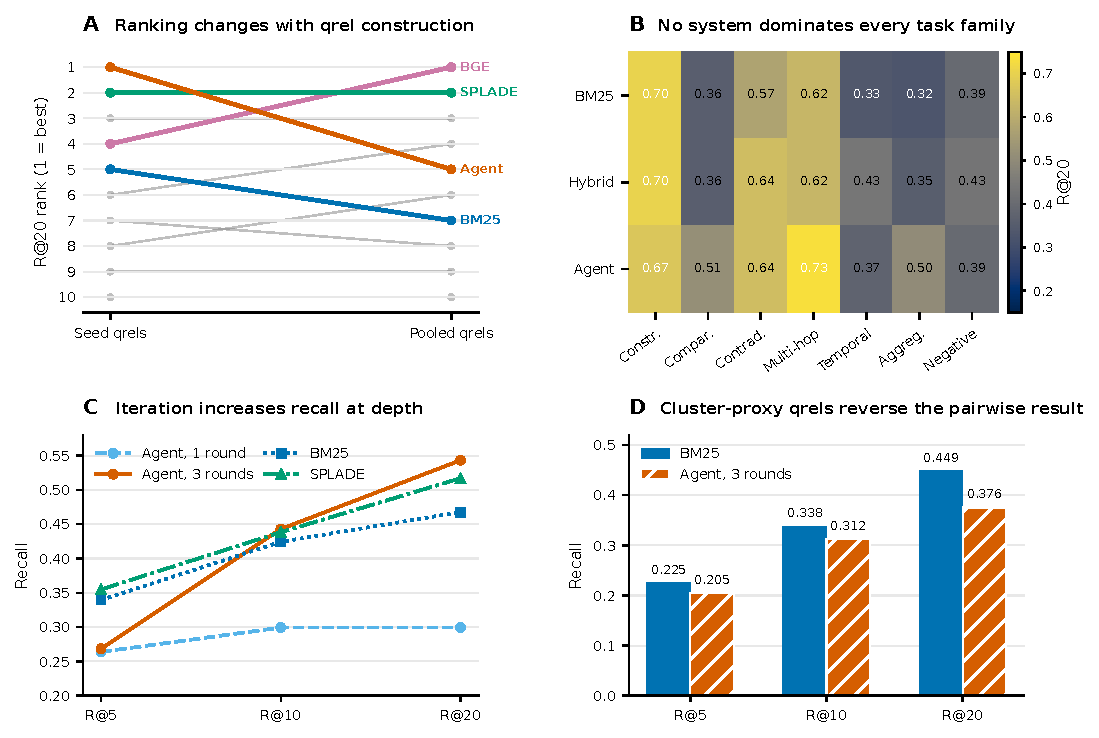
\includegraphics[width=\textwidth]{figures/label_sensitivity_analysis.pdf}
  \caption{Four views of conclusion stability. \textbf{A}: R@20 ranks for ten systems under seed versus pooled qrels; highlighted systems illustrate the principal changes. Absolute recall values are not compared across regimes because their denominators differ. \textbf{B}: v1 R@20 by family for representative lexical, fused, and iterative systems. \textbf{C}: one- versus three-round agent ablation with BM25 and SPLADE references. \textbf{D}: BM25 and the three-round agent on 70 v2 test tasks with cluster-proxy qrels. Numeric source data and plotting code are regenerated by the submission audit.}
  \label{fig:robustness}
\end{figure*}

\subsection{Qrel Sensitivity Changes the Headline}

Under pooled qrels, BGE has the highest R@20 (0.416), followed by SPLADE (0.388), hybrid retrieval (0.377), and E5-large (0.362); the agent falls to fifth (0.352). Pooling credits documents found by single-pass systems that were absent from the seed set. The result does not prove that BGE is best under human relevance; it shows that the agent's seed-qrel lead is not stable to broader LLM adjudication.

The v2 cluster-proxy comparison points in the same directional sense but is narrower: on 70 test tasks, BM25 exceeds the agent at R@5 (0.225 vs.\ 0.205), R@10 (0.338 vs.\ 0.312), and R@20 (0.449 vs.\ 0.376). Only these two v2 retrieval outputs are bundled, so no claim is made about all-method v2 ordering. Figure~\ref{fig:robustness}A,D summarizes both shifts.

Family results remain heterogeneous (Figure~\ref{fig:robustness}B). On v1 R@20, the agent leads or ties on contradiction, multi-hop, comparison, and aggregation, while BM25 or hybrid retrieval lead on constraints, temporal questions, and negative results. These subsets are small and the seed qrels are construction-dependent, so the family matrix is diagnostic rather than confirmatory.

\subsection{Abstention and Split Sensitivity}

Every evaluated retrieval configuration returns documents for all 17 unsupported queries; none implements a calibrated abstention decision. A saved gradient-boosted diagnostic using cross-method agreement, query length, and constraint count obtains AUROC 0.698 and AUPRC 0.222 across 17 positive and 108 negative cases. This is a post-hoc diagnostic, not a deployed abstention method, and its small positive sample makes the estimate uncertain.

On the 82 non-abstention test tasks whose supporting documents do not occur in train or development, the qualitative depth result persists: R@20 is 0.565 for the agent, 0.547 for SPLADE, 0.510 for hybrid retrieval, and 0.482 for BM25. At shallower ranks SPLADE leads (R@10 0.474 vs.\ agent 0.457). The slice removes known document overlap but does not remove topic or template similarity.

\section{Discussion and Conclusion}
\label{sec:conclusion}

\cer demonstrates two distinct sources of variance in scientific retrieval evaluation. The first is \emph{capability structure}: lexical, sparse, fused, and iterative systems lead on different families and rank depths. The second is \emph{qrel construction}: changing which documents receive relevance credit reverses the aggregate conclusion. Reporting a single leaderboard number would obscure both.

The current benchmark has substantial limitations. Seed qrels are generated from the same papers used to write each query; pooled judgments reuse the generator's model family; cluster-proxy qrels over-credit topic-cluster membership; and no independent biomedical annotators have validated relevance. The corpus is small, English-only, biomedical-only, and predominantly abstract-only. Splits are not document-disjoint, two questions repeat across train and test, the controller uses a proprietary backbone and only BM25 tools, and the evaluated rerankers are not biomedical-specific. We therefore do not present \cer as a definitive leaderboard or as a clinical benchmark.

Within those bounds, the evidence supports three conclusions. Iterative reformulation reliably improves the same controller's recall at depth under seed qrels. Strong single-pass systems remain competitive and often preferable in cost, latency, and ranking precision. Most importantly, retrieval claims should be accompanied by relevance-judgment provenance and sensitivity analysis. Future releases should prioritize blinded human pooling, document- and cluster-disjoint splits, explicit structural annotations, and calibrated selective retrieval before increasing model scale.
\label{page:mainend}

\section*{AI use statement}
Generative AI was used to generate corpus-grounded benchmark questions, execute the evaluated iterative controllers, filter v2 topic clusters, and adjudicate pooled candidate documents. It also assisted with experimental auditing, reference checking, scientific-figure planning, plotting-code development, and manuscript editing. The paper identifies the relevant model versions, prompts, and limitations in Sections~\ref{sec:qrels}--\ref{sec:results} and Appendices~\ref{app:generation}, \ref{app:controller}, and~\ref{app:pooling}. The authors reviewed the saved artifacts, regenerated paper-facing metrics and figures with deterministic scripts, and take responsibility for the final text, claims, code, and data. No generative-AI output is treated as independent human validation.

\section*{Ethics statement}
The source corpus consists of public scholarly records and licensed open-access articles; it contains no patient records or direct study-participant data. Biomedical retrieval errors can nevertheless create false confidence. We therefore include unsupported queries, report that no tested system abstains, and prohibit interpreting \cer scores as evidence of clinical safety or suitability for medical decision support. The review supplement excludes raw abstract and full-text corpora; Appendix~\ref{app:governance} documents the distributed fields and remaining licensing caveats.

\section*{Reproducibility statement}
The review supplement contains sanitized task metadata, saved score summaries, the numerical integrity audit, plotting code, controller prompts, and LaTeX source. \texttt{scripts/31\_submission\_audit.py} recomputes corpus and split counts, v1 and v2 headline metrics, pooled-adjudication counts, document-overlap statistics, and paired-bootstrap intervals from saved artifacts; \texttt{scripts/32\_make\_submission\_figure.py} regenerates Figure~\ref{fig:robustness}; and \texttt{scripts/run\_iclr2027\_submission.sh} rebuilds and checks the PDF. Appendix~\ref{app:repro} lists exact model identifiers, software assumptions, and which expensive API/model runs are not repeated by the paper build.

\bibliographystyle{iclr2027_conference}
\bibliography{refs}

\newpage
\appendix

\section{Corpus Construction and Statistics}
\label{app:corpus}

PubMed E-utilities supplies identifiers, titles, abstracts, MeSH terms, publication types, and dates. OpenAlex enrichment adds citation links, concepts, topics, venue metadata, and open-access status. For the 652 records with eligible PMC XML, section headings are mapped to scientific section types; figure captions and table text are extracted separately. Abstracts are capped at 512 estimated tokens, sections at 1,024, and captions and table text at 256 and 512. Table~\ref{tab:corpusstats} records the resulting corpus.

\begin{table}[h]
\centering
\caption{Corpus statistics recomputed from \texttt{corpus\_stats.json}.}
\label{tab:corpusstats}
\small
\begin{tabular}{lr}
\toprule
Statistic & Value \\
\midrule
Documents & 4,936 \\
PMC full text & 652 (13.2\%) \\
Abstract-only & 4,284 (86.8\%) \\
Chunks & 17,902 \\
Estimated tokens & 6,591,919 \\
Median / mean chunk length & 304 / 368 \\
Year range & 2015--2026 \\
Seed subdomains & 10 \\
\bottomrule
\end{tabular}
\end{table}

\begin{table}[h]
\centering
\caption{Exact document counts by seed search after cross-query deduplication.}
\label{tab:subdomains}
\small
\begin{tabular}{lr@{\qquad}lr}
\toprule
Subdomain & $n$ & Subdomain & $n$ \\
\midrule
Microbiome/disease & 500 & Protein structure & 500 \\
Single-cell methods & 499 & mRNA therapeutics & 497 \\
Drug repurposing & 496 & Organoid models & 495 \\
Epigenetics/disease & 495 & CAR-T therapy & 493 \\
Checkpoint therapy & 492 & CRISPR methods & 469 \\
\bottomrule
\end{tabular}
\end{table}

\section{Task Details, Prompts, and Examples}
\label{app:taskdetails}
\label{app:generation}

Table~\ref{tab:splits} gives exact split counts. Generation uses Claude Sonnet 4 (\texttt{claude-sonnet-4-20250514}) at temperature 0.7. For each family the model receives the sampled papers' identifiers, titles, abstracts, years, venues, and MeSH terms. The prompt requires exact constraints from the provided context and a JSON object containing the question, difficulty, structured constraints, expected answer type, and reference answer.

\begin{table}[h]
\centering
\caption{Tasks by family and split.}
\label{tab:splits}
\small
\begin{tabular}{lrrrr}
\toprule
Family & Train & Dev & Test & Total \\
\midrule
Constraint & 15 & 8 & 15 & 38 \\
Comparative & 15 & 8 & 15 & 38 \\
Contradiction & 16 & 8 & 14 & 38 \\
Abstention & 14 & 7 & 17 & 38 \\
Multi-hop & 15 & 7 & 16 & 38 \\
Temporal & 14 & 7 & 17 & 38 \\
Aggregation & 14 & 7 & 17 & 38 \\
Negative & 16 & 8 & 14 & 38 \\
\midrule
Total & 119 & 60 & 125 & 304 \\
\bottomrule
\end{tabular}
\end{table}

Representative family instructions are:
\begin{quote}\small
\textbf{Constraint:} Generate a question requiring 2--4 specific experimental constraints. Only papers satisfying all constraints should support the question.\\
\textbf{Comparative:} Generate a question requiring evidence from both comparison groups; retrieving one side is insufficient.\\
\textbf{Abstention:} Generate a plausible question related to the supplied papers but combining constraints that none satisfies jointly.\\
\textbf{Aggregation:} Generate a question asking for all reported values or findings for a defined measurement or outcome.
\end{quote}

Example questions include: \emph{``Compare targeted genome modification in C.~elegans and mammalian systems using CRISPR-Cas9 delivery strategies''} (comparative); \emph{``How has the understanding of epigenetic mechanisms in cancer evolved from histone-modification cataloging to therapeutic targeting?''} (temporal); and \emph{``What reported IC50 values exist for palbociclib across cancer cell lines and assay conditions?''} (aggregation). An abstention example asks for a pediatric Chagas-cardiomyopathy comparison absent from the corpus. These examples illustrate intended form, not independent proof that all assigned qrels satisfy every constraint.

\section{Controller Architecture and Prompt}
\label{app:controller}

The exact system prompt is:
\begin{verbatim}
You are a scientific literature retrieval agent.
Find the most relevant papers for the research question.

Actions:
SEARCH(query): execute a corpus query.
REFINE(reasoning, query): target missing constraints.
STOP(selected_docs, reasoning): return final evidence.

Process:
1. Identify organism, method, condition, and outcome.
2. Search with the full question.
3. Evaluate which constraints the evidence satisfies.
4. Refine for important unsatisfied constraints.
5. Stop when evidence is sufficient or the budget ends.

Return one JSON action only.
\end{verbatim}

At temperature 0, the controller performs at most three calls. Each search result contains a document title and a 120-character text snippet. Previously seen chunks are excluded from subsequent rounds. If no explicit stop occurs by round three, accumulated unique documents are returned in first-retrieval order, capped at 20.

\section{Full Family Results}
\label{app:family}

\begin{table}[h]
\centering
\caption{V1 Recall@10 by non-abstention family. Best among shown systems is bold.}
\label{tab:r10family}
\small
\begin{tabular}{lrrrrrr}
\toprule
Family & BM25 & SPECTER2 & BGE & Hybrid & Hybrid+CE & Agent \\
\midrule
Constraint & \textbf{.633} & .233 & .567 & .567 & .333 & .600 \\
Multi-hop & \textbf{.583} & .292 & .500 & .417 & .292 & .521 \\
Contradiction & .536 & .429 & .429 & \textbf{.607} & .429 & .571 \\
Negative & .357 & .393 & \textbf{.464} & .429 & .429 & .393 \\
Comparative & \textbf{.356} & .178 & .222 & .267 & .156 & \textbf{.356} \\
Aggregation & .324 & .206 & .265 & .353 & .176 & \textbf{.412} \\
Temporal & .216 & .098 & .235 & \textbf{.314} & .078 & .275 \\
\bottomrule
\end{tabular}
\end{table}

\begin{table}[h]
\centering
\caption{V1 Recall@20 by non-abstention family. ``Dense'' denotes SPECTER2 and ``Hybrid+CE'' the MS-MARCO reranker.}
\label{tab:r20family}
\small
\begin{tabular}{lrrrrr}
\toprule
Family & BM25 & Dense & Hybrid & Hybrid+CE & Agent \\
\midrule
Constraint & \textbf{.700} & .367 & \textbf{.700} & .500 & .667 \\
Contradiction & .571 & .500 & \textbf{.643} & .536 & \textbf{.643} \\
Multi-hop & .625 & .417 & .625 & .396 & \textbf{.729} \\
Negative & .393 & \textbf{.500} & .429 & .464 & .393 \\
Aggregation & .324 & .235 & .353 & .235 & \textbf{.500} \\
Comparative & .356 & .222 & .356 & .222 & \textbf{.511} \\
Temporal & .333 & .216 & \textbf{.431} & .216 & .373 \\
\bottomrule
\end{tabular}
\end{table}

\section{Pooled Adjudication}
\label{app:pooling}

The candidate pool unions top-20 document results from BM25, SPECTER2, BGE, E5-large, MedCPT, SPLADE, hybrid RRF, hybrid+MS-MARCO CE, BM25+BGE-reranker, and the three-round agent. BM25+RM3 is excluded because of high overlap with BM25. Seed qrels are automatically retained; all other pooled pairs are judged blind to contributing method and rank. The binary rubric requires every stated constraint and an explicit supporting span. Saved strings are normalized by trimming whitespace, converting to uppercase, and testing the \texttt{NOT\_RELEVANT} prefix before \texttt{RELEVANT}; no record is unparseable under this rule.

\begin{table}[h]
\centering
\caption{Recall under pooled qrels (108 tasks; mean 12.7 qrels/query). These values are not numerically comparable with seed-qrel recall because the denominators differ.}
\label{tab:pooled}
\small
\begin{tabular}{lrr}
\toprule
Method & R@10 & R@20 \\
\midrule
BM25 & .251 & .321 \\
SPECTER2 & .197 & .302 \\
BGE & \textbf{.294} & \textbf{.416} \\
E5-large & .262 & .362 \\
MedCPT & .181 & .275 \\
SPLADE & .276 & .388 \\
Hybrid & .291 & .377 \\
Hybrid+MS-MARCO CE & .219 & .336 \\
BM25+BGE-reranker & .245 & .319 \\
Agent ($T{=}3$) & .274 & .352 \\
\bottomrule
\end{tabular}
\end{table}

The pooled set has a participation bias: only documents retrieved by contributing systems can be judged. The use of the same Sonnet model family for generation and judging may introduce correlated preferences. Supporting-span requirements and method/rank blinding reduce, but do not remove, these threats.

\section{Cluster-Proxy Qrels (v2)}
\label{app:v2}

The v2 generation script first retrieves BM25 neighbors of a seed paper using its title and abstract. Sonnet then selects candidates related to the \emph{seed topic}; the prompt does not yet contain the final query. A second Sonnet call generates the query from up to twelve cluster papers, after which all 6--16 cluster members are assigned to the qrel set. Several reference answers mention only a subset of assigned members, directly demonstrating why cluster membership cannot be interpreted as document-level verification against the final query.

Across the 200 tasks, non-empty clusters average 9.81 assigned documents (range 6--16). The 70 non-abstention test tasks with saved agent outputs have BM25/agent scores of .225/.205 R@5, .338/.312 R@10, .449/.376 R@20, .391/.361 nDCG@10, and .675/.667 MRR. BM25 is rerun from the saved exact index by the submission-audit script; agent results are read from \texttt{data/benchmark/v2/agent\_test.jsonl}.

\section{Split-Integrity and Document-Disjoint Sensitivity}
\label{app:split}

The v1 split is stratified by family only. Train and development share 17 supporting documents, train and test share 35, and development and test share 14. Twenty-six test tasks share at least one supporting document with train or development. Exact query normalization finds two train--test duplicates, both temporal questions. These facts do not contaminate unsupervised index construction, which uses the same corpus for all methods, but they matter for prompt development and any future supervised training.

\begin{table}[h]
\centering
\caption{Sensitivity on 82 non-abstention test tasks with no supporting document in train or development.}
\label{tab:disjoint}
\small
\begin{tabular}{lrrrrr}
\toprule
Method & R@5 & R@10 & R@20 & nDCG@10 & MRR \\
\midrule
BM25 & .360 & .453 & .482 & .413 & .581 \\
SPLADE & \textbf{.376} & \textbf{.474} & .547 & \textbf{.437} & \textbf{.592} \\
Hybrid & .356 & .435 & .510 & .383 & .529 \\
Agent ($T{=}3$) & .268 & .457 & \textbf{.565} & .370 & .514 \\
\bottomrule
\end{tabular}
\end{table}

This post-hoc slice preserves the agent's descriptive R@20 lead but makes SPLADE strongest at R@5, R@10, nDCG@10, and MRR. A future benchmark revision should rebuild all splits at the document-cluster level before task generation rather than filter after evaluation.

\section{Paired Bootstrap Comparisons}
\label{app:stats}

For each pair, we compute the per-task recall difference, sample 108 tasks with replacement 10,000 times using NumPy's generator with seed 42, and take the 2.5th and 97.5th percentiles. Two-sided bootstrap tail probabilities are provided by the audit but confidence intervals are emphasized because several comparisons are exploratory.

\begin{table}[h]
\centering
\caption{Agent ($T{=}3$) minus comparator on v1.}
\label{tab:bootstrap}
\small
\begin{tabular}{llrr}
\toprule
Metric & Comparator & Mean $\Delta$ & 95\% CI \\
\midrule
R@10 & BM25 & .019 & [$-.025$, .063] \\
R@10 & SPLADE & .005 & [$-.046$, .057] \\
R@10 & Hybrid & .026 & [$-.019$, .069] \\
R@10 & Agent $T{=}1$ & .144 & [.107, .184] \\
R@20 & BM25 & .076 & [.031, .122] \\
R@20 & SPLADE & .026 & [$-.032$, .085] \\
R@20 & Hybrid & .042 & [$-.006$, .090] \\
R@20 & Agent $T{=}1$ & .244 & [.196, .296] \\
\bottomrule
\end{tabular}
\end{table}

\section{Abstention Diagnostics}
\label{app:abstention}

All primary systems return non-empty rankings on every task, so retrieval metrics cannot by themselves represent abstention. The saved diagnostic labels the 17 empty-qrel queries as positives and 108 supported queries as negatives. Features include query length, number of structured constraints, top-result agreement across methods, top-10 pool overlap, and the number of unique top-10 documents. Five-fold stratified cross-validation of a gradient-boosted classifier yields AUROC .698, AUPRC .222, F1 .250, and area under the risk--coverage curve .067. With only 17 positives, no separately held-out benchmark, and family-templated query features, these numbers establish feasibility of selective-retrieval analysis rather than a reliable abstention baseline.

\section{Cost, Latency, and Exploratory Backbone Swap}
\label{app:cost}

\begin{table}[h]
\centering
\caption{Saved engineering estimates per query. Local marginal cost excludes hardware acquisition and index construction.}
\label{tab:cost}
\small
\begin{tabular}{lrrl}
\toprule
Method & Latency & Marginal cost & Infrastructure \\
\midrule
BM25 & 0.3 s & negligible & CPU \\
Dense & 0.5 s & $\sim\$0.0001$ & GPU+CPU \\
Hybrid & 0.6 s & $\sim\$0.0001$ & GPU+CPU \\
Hybrid+CE & 1.2 s & $\sim\$0.0002$ & GPU+CPU \\
Agent $T{=}1$ & 5.7 s & $\$0.03$ & CPU+LLM API \\
Agent $T{=}3$ & 17.2 s & $\$0.08$ & CPU+LLM API \\
\bottomrule
\end{tabular}
\end{table}

The three-round agent is about 57 times slower than local BM25 in these saved estimates. A multiplicative cost comparison is undefined because BM25's recorded marginal query cost is zero.

An exploratory GPT-5.4 controller run covers 65 non-abstention tasks also evaluated by Sonnet. On this subset, GPT-5.4/Sonnet obtain .349/.349 R@5, .436/.492 R@10, .480/.560 R@20, .416/.385 nDCG@10, and .524/.478 MRR. No independently reproducible significance artifact accompanies this subset, so we report it descriptively and do not use it to claim absence of generator--controller leakage.

\section{Reproducibility and Artifact Inventory}
\label{app:repro}

The deterministic review workflow is:
\begin{verbatim}
python scripts/31_submission_audit.py
python scripts/32_make_submission_figure.py
bash scripts/run_iclr2027_submission.sh
\end{verbatim}
The audit reads the JSONL task splits, saved top-20 retrieval outputs, expanded pooled qrels, adjudication records, v2 tasks and agent outputs, corpus statistics, and saved BM25 index. It writes \texttt{results/paper\_tables/submission\_audit.json}. The plotting script consumes that audit and the comprehensive v1 score file to export PDF, SVG, 600-dpi PNG, and grayscale-QA versions of Figure~\ref{fig:robustness}. The shell entry point then compiles the official ICLR 2027 source, rejects unresolved citations/references, checks the nine-page marker, and verifies embedded fonts.

Exact model identifiers are: \path{allenai/specter2_base} with the \path{allenai/specter2} proximity adapter; \path{BAAI/bge-base-en-v1.5}; \path{intfloat/e5-large-v2}; MedCPT query/article encoders; \path{naver/splade-cocondenser-ensembledistil}; \path{cross-encoder/ms-marco-MiniLM-L-12-v2}; \path{BAAI/bge-reranker-v2-m3}; and \path{claude-sonnet-4-20250514}. BM25 uses lowercase alphanumeric tokenization, $k_1{=}1.2$, and $b{=}0.75$. Retrieval is deterministic; task generation uses temperature 0.7 and the controller and judge use temperature 0.

The paper build does not rerun commercial-API generation, LLM judging, neural indexing, or agent inference. It verifies claims against saved outputs. The supplement intentionally omits unsupported trained-controller claims, Croissant-validation claims, and human-agreement statistics present in an earlier draft because matching artifacts do not exist.

\section{Data Governance and Review Supplement}
\label{app:governance}

The review supplement contains questions, constraints, family labels, splits, supporting identifiers, hard-negative identifiers, result summaries, audit outputs, scripts, and paper source. It removes \texttt{supporting\_passages} before packaging and does not distribute the raw corpus, PubMed abstracts, PMC XML, local absolute paths, credentials, model caches, or author-identifying metadata. This supports anonymous review while avoiding a blanket redistribution claim for abstract text.

PMC full text remains governed by each article's license; PubMed records can contain publisher-copyrighted abstracts; OpenAlex metadata has separate terms. A public benchmark release therefore requires a per-record license manifest and a re-fetch workflow reviewed by the authors. Until that legal and provenance review is complete, the supplement should be treated as a review artifact rather than a fully licensed public dataset release.

\end{document}
